%%%%%%%%%%%%%%%%%%%%%%%%%%%%%%%%%%%%%%%%%%%%%%%%%%%%%%%%%%%%%%%%%%%%%%%%%%%%%%%%%%%
\section{Logarithmische Darstellung, Frequenzgang, Grenzfrequenz}
\label{sec:frequenzganglog}%
\begin{frame}\ftx{\secname}%
\s{\index{logarithmische Darstellung}%
    % Einleitung
    In der Elektrotechnik und Nachrichtentechnik werden häufig logarithmische Skalen verwendet,
    um den Frequenzgang von Filtern und Verstärkern darzustellen. Die logarithmische Darstellung
    ermöglicht eine bessere Übersicht über das Verhalten des Systems im gesamten Frequenzbereich.

    Abbildung \ref{fig:xkcd_logscale} zeigt zwei Comic-Strips von XKCD, die die Vorteile der logarithmischen
    Darstellung humorvoll darstellen.

    In diesem Kapitel werden wir uns mit der logarithmischen Darstellung von Frequenzgängen in Form sogenannter
    Bode-Diagramme beschäftigen. Zur Beschreibung des Frequenzganges einfacher Filterschaltungen werden
    die Einheit Dezibel, sowie die Grenzfrequenz und die Ordnung von Filtern definiert.
    Darüber hinaus werden Bandpass- und Bandsperrfilter vorgestellt.
}%
\begin{Lernziele}{Logarithmische Darstellung, Frequenzgang}
    Studierende lernen:
    \begin{itemize}
        \item Unterschiede zwischen linearer und logarithmischer Darstellung kennen.
        \item Dezibel als Einheit kennen und zu verwenden.
        \item Grenzfrequenzen von Filterschaltungen kennen und zu bestimmen.
        \item Bodediagramme zu konstruieren und zu interpretieren.
        \item Funktionsweise von Bandpass- und Bandsperrfilter kennen und verstehen.
        \item Aufbau und Verhalten von Filtern höherer Ordnung kennen und verstehen. 
    \end{itemize}
\end{Lernziele}
\end{frame}%

\begin{frame}\ftx{\secname}%
% <--- here is an empty page (Skript), dunno why... o.o, disappears if surrounding \begin{frame}...\b{...}\end{frame} is commented out --->
\s{% single page comic strips (left and right)
    \begin{figure}[H]
        \begin{subfigure}{.5\textwidth}\centering% left
            \resizebox{!}{.95\textheight}{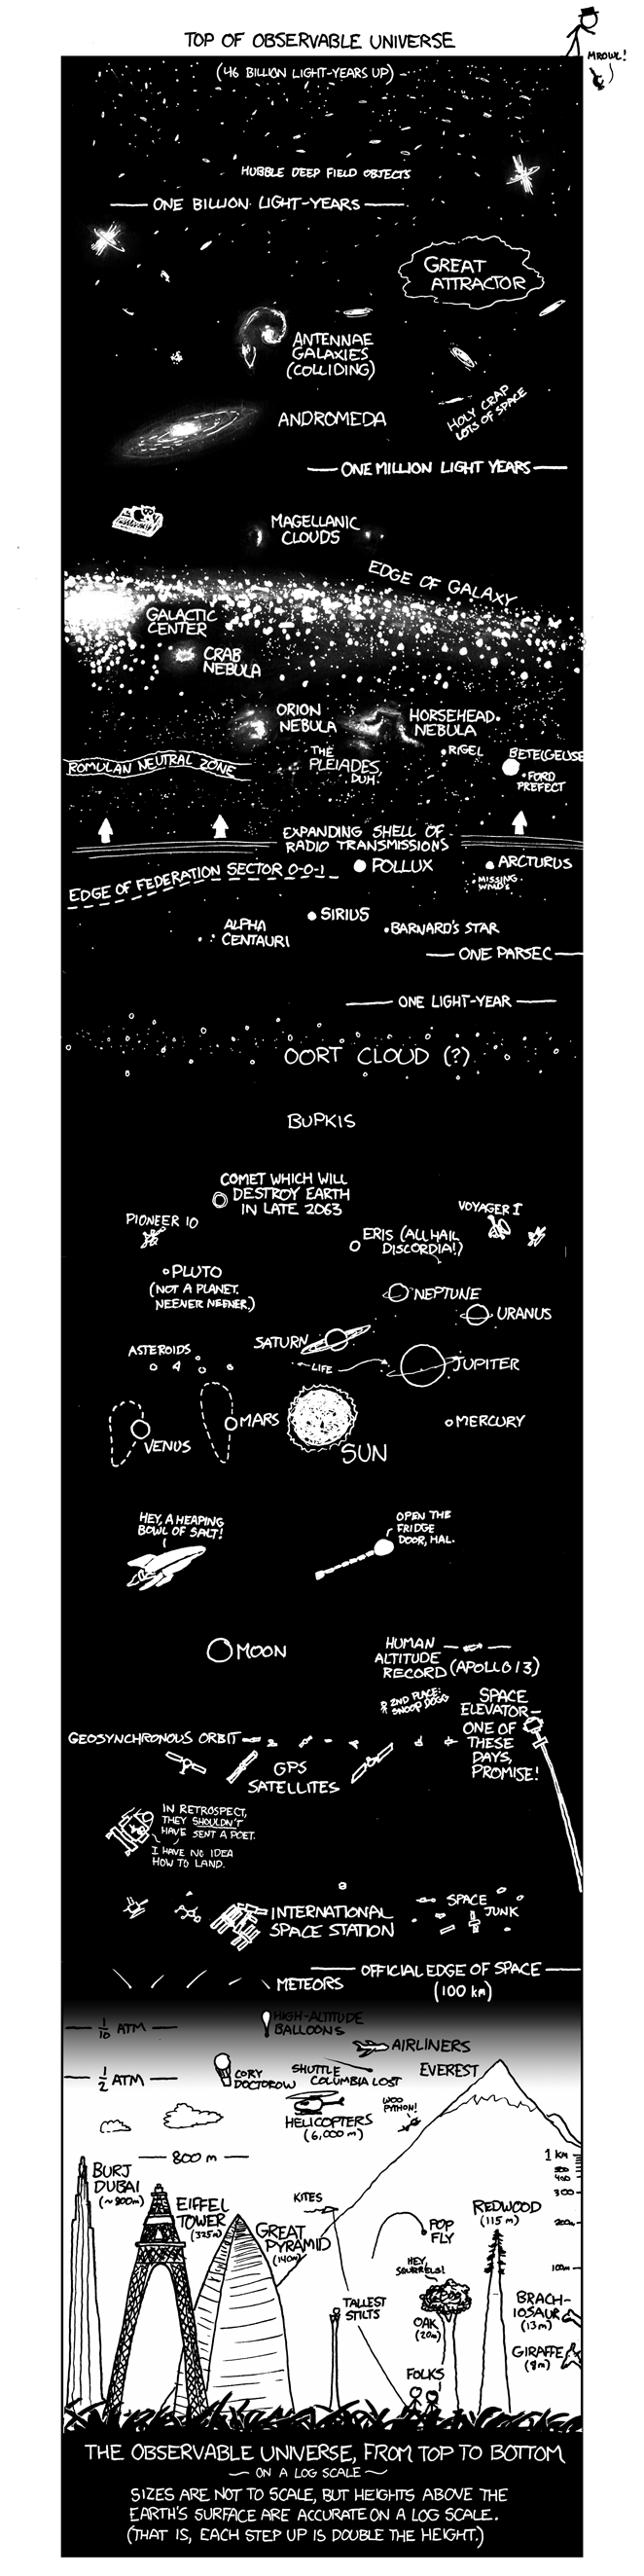
\includegraphics{Bilder/xkcd_482_height_logaxis_large_scales_cc-2.5-by-sa.png}}
                \caption{Comic \textit{Height}, Log-Skala Höhe\cite[\#482]{xkcd}}%
        \end{subfigure}%
        \begin{subfigure}{.5\textwidth}\centering% right
            \resizebox{!}{.95\textheight}{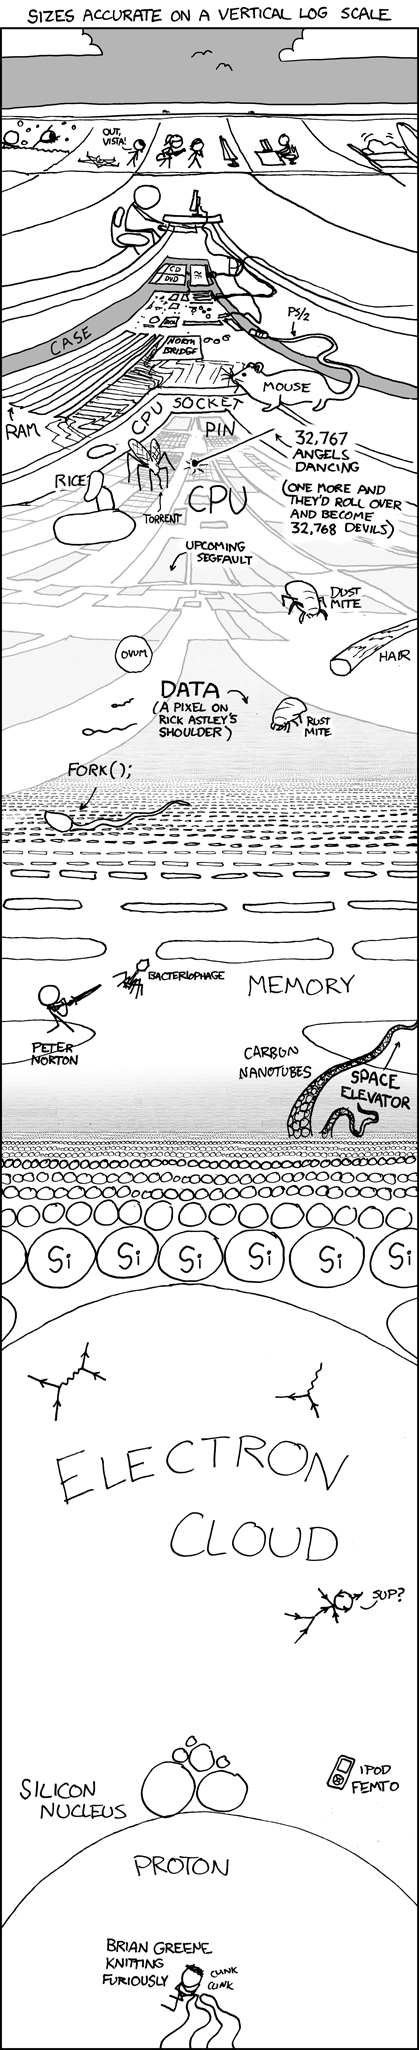
\includegraphics{Bilder/xkcd_485_depth_logaxis_small_scales_cc-2.5-by-sa.png}}
                \caption{Comic \textit{Depth}, Log-Skala Tiefe\cite[\#485]{xkcd}}%
        \end{subfigure}\hfill
        \caption{xkcd Comics zu logarithmischen Darstellungen von Größen}%
        \label{fig:xkcd_logscale}%
    \end{figure}
}%
\b{%
\begin{columns}% multi-slide comic strips (left column, right column) with overlays
    \column[c]{0.5\textwidth}%
        \only<beamer:1-3| handout:1-3>{\resizebox{!}{\textheight}{% beware: \resizebox without content -> Division by 0 error
            % animation with            trim={left bottom right top}
            \only<beamer:1| handout:1>{\adjincludegraphics[trim={0 {0.650\height} 0 {0.000\height}},clip]{Bilder/xkcd_482_height_logaxis_large_scales_cc-2.5-by-sa.png}}%
            \only<beamer:2| handout:2>{\adjincludegraphics[trim={0 {0.325\height} 0 {0.325\height}},clip]{Bilder/xkcd_482_height_logaxis_large_scales_cc-2.5-by-sa.png}}%
            \only<beamer:3| handout:3>{\adjincludegraphics[trim={0 {0.000\height} 0 {0.650\height}},clip]{Bilder/xkcd_482_height_logaxis_large_scales_cc-2.5-by-sa.png}}% 
        }}% %Note: Bei 66% Schnitt, 34% Anzeige trotz 2x0.5% Overlap Teile des Bildes in Frame abgeschnitten, daher 65% Schnitt, 35% Anzeige, 2x1% Overlap
        \only<beamer:4-5| handout:4-5>{
            \vskip.75\textheight% \vspace{\fill} not working, \null\vfill not working, ~\vfill not working
            \tiny Quelle: xkcd \#482, \textit{Height}, \url{https://xkcd.com/482/} (Abruf: 04.04.2024)}%
    \column[c]{0.5\textwidth}%
        \only<beamer:3-5| handout:3-5>{\resizebox{!}{\textheight}{% beware: \resizebox without content -> Division by 0 error
            % animation with            trim={left bottom right top}
            \only<beamer:3| handout:3>{\adjincludegraphics[trim={0 {0.650\height} 0 {0.000\height}},clip]{Bilder/xkcd_485_depth_logaxis_small_scales_cc-2.5-by-sa.png}}
            \only<beamer:4| handout:4>{\adjincludegraphics[trim={0 {0.325\height} 0 {0.325\height}},clip]{Bilder/xkcd_485_depth_logaxis_small_scales_cc-2.5-by-sa.png}}
            \only<beamer:5| handout:5>{\adjincludegraphics[trim={0 {0.000\height} 0 {0.650\height}},clip]{Bilder/xkcd_485_depth_logaxis_small_scales_cc-2.5-by-sa.png}}
        }}%
        \only<beamer:1-2| handout:1-2>{Multipage Comic Strip (vertikal Scrollen)%
            \vskip.75\textheight% \vspace{\fill} not working, \null\vfill not working, ~\vfill not working
            \tiny Quelle: xkcd \#482, \textit{Depth}, \url{https://xkcd.com/485/} (Abruf: 04.04.2024)}%
\end{columns}%
}%
\end{frame}%

%%%%%%%%%%%%%%%%%%%%%%%%%%%%%%%%%%%%%%%%%%%%%%%%%%%%%%%%%%%%%%%%%%%%%%%%%%%%%%%%%%%

\subsection{Logarithmische Darstellung von Potenzfunktionen}
\label{sec:frequenzganglog:potenzfunktionen}
\begin{frame}\ftx{\subsecname}
    \s{
        In der logarithmischen Darstellung wird eine logarithmische Skala für eine oder mehrere Achsen verwendet.
        Eine lineare Zunahme von abzubildenden Werten korrespondiert hierbei mit einer logarithmischen Zunahme der Distanz auf der Skala.
        Anschaulicher im Umkehrschluss: 
        Bei linearer Zunahme der Distanz auf der Skala steigt die Potenz der abzubildenden Werte im selben Maß linear an. 
        
        %Lineare Wertezunahme -> Logarithmische Achsenschritte
        %Potenzierende Wertezunahme -> Lineare Achsenschritte
        %Dies bedeutet bei linearer Zunahme eines Wertes, ergibt sich ein logarthmischer Zuwachs (des Abstandes) auf der Achse.
        %Daraus folgt, dass sich bei potenzierender Zunahme eines Wertes ein linearer Anstieg auf der Achse ergibt.  

        Logarithmische Skalen bieten sich im Allgemeinen an, um Wertebereiche über mehrere Größenordnungen darzustellen.
        Eine Besonderheit in der doppelt logarithmischen Darstellung ist, dass Potenzfunktionen als Geraden dargestellt werden.
        Abbildung \ref{fig:vgl:potenzfunktionen:lin:log} zeigt zum Vergleich mehrerer Potenzfunktionen in linearer Darstellung (links)
        und in doppelt-logarithmischer Darstellung mit Basis\ $10$ (rechts).

        \begin{figure}[H]
            \begin{subfigure}{0.48\textwidth}\centering
                \resizebox*{\textwidth}{!}{\includegraphics{Tikz/pdf/plot_potenzfunktionen_lin_scale.pdf}}
                \caption{Potenzfunktionen, lineare Achsen}
            \end{subfigure}%
            \begin{subfigure}{0.48\textwidth}\centering
                \resizebox*{\textwidth}{!}{\includegraphics{Tikz/pdf/plot_potenzfunktionen_log_scale.pdf}}
                \caption{Potenzfunktionen, logarithmische Achsen}
            \end{subfigure}\hfill
            \caption{Vergleich lineare und logarithmische Skalierung von Potenzfunktionen}
            \label{fig:vgl:potenzfunktionen:lin:log}
        \end{figure}%
        Der Exponent einer Potenzfunktion entspricht in doppelt-logarithmischer Darstellung der Steigung der Geraden.
        Eine Verschiebung in y-Richtung entspricht einem Vorfaktor $a$ für die Funktion $f(x)$,
        eine Verschiebung in x-Richtung einem Vorfaktor $x_{\mathrm{off}}$ für x in der Funktion. 
        Durch diese Eigenschaften eignet sich die logarithmische Darstellung besonders zur Darstellung von Amplitudengängen.
    }%
    \b{
        \begin{columns}
            \column[c]{0.5\textwidth}\resizebox*{\textwidth}{!}{
                \includegraphics{Tikz/pdf/plot_potenzfunktionen_lin_scale.pdf}}
                \centering \textbf{Lineare Darstellung}
                \begin{itemize}
                    \item Gerade: $\ f(x) = a \left(x-x_{0}\right) + y_{0}$
                    \item Add./Subtr. $\rightarrow$ Verschiebung %
                    \item Mult./Div. $\rightarrow$ Streckung%
                    %\item negative x-Werte möglich
                \end{itemize}
            \column[c]{0.5\textwidth}\resizebox*{\textwidth}{!}{
                \includegraphics{Tikz/pdf/plot_potenzfunktionen_log_scale.pdf}}
                \centering \textbf{(Doppelt-)Logarithmische Darstellung}
                \begin{itemize}
                    \item Gerade: $\ f(x) =  \left({x}/{x_{0}}\right)^{\displaystyle a} \cdot y_{0}$
                    \item Mult./Div. $\rightarrow$ Verschiebung
                    \item Exponent $\rightarrow$ Streckung
                    %\item keine negativen log. Werte für reelle x, y
                \end{itemize}
        \end{columns}
    }
\end{frame}
%%%%%%%%%%%%%%%%%%%%%%%%%%%%%%%%%%%%%%%%%%%%%%%%%%%%%%%%%%%%%%%%%%%%%%%%%%%%%%%%%%%%%%%%%%%%%%%%%%%

\subsection{Definition Dezibel}
\label{sec:frequenzganglog:dezibel}
\begin{frame}\ftx{\subsecname}
\s{%
    \index{Dezibel}%
    Dezibel ist eine Hilfsmaßeinheit zur Kennzeichnung dekadisch-logarithmischer Verhältnisse zweier Größen.
    Verwendung findet es u.A. in der Signaltheorie und Nachrichtentechnik, beispielsweise um die Verstärkung/Dämpfung 
    eines Bauteils oder einer Signalstrecke anzugeben. Ein Dezibel $[\mathrm{\dB}]$ entspricht dem zehnfachen der Basiseinheit Bel $[\mathrm{B}]$. 
    %welche nach Alexander Graham Bell benannt ist.\cite{QUELLE}

    Definiert ist das Bel als Kennzeichnung des dekadisch-logarithmischen Verhältnisses (Symbol $Q$) zweier einheitengleicher Leistungsgrößen (Index $P$)
    wie in Gleichung \ref{eq:def:dezibel:leistung} gezeigt ist. %QUELLE
    In Zusammenhang mit Spannung oder Strom als sogenannte Leistungswurzelgrößen (ehemals Feldgrößen, Index $F$) 
    kann das (Dezi-)Bel in linearen Systemen ebenfalls verwendet werden wie in Gleichung \ref{eq:def:dezibel:wurzel} gezeigt ist.
    Die Umrechnung basiert auf der Proportionalität von $P\sim U^2$ beziehungsweise $P\sim I^2$, woraus sich der Faktor $2$ ergibt.%

	\begin{align}% script only - with numbering
        &\textrm{Leistungsgrößen }(\textrm{z.B. }P,\ W)&
            Q_{\mathrm{(P)}} &= \mathrm{log}\frac{P_2}{P_1}\ \operatorname{B} = 10\cdot \mathrm{log}\frac{P_1}{P_2}\ \dB &&
            \label{eq:def:dezibel:leistung}\\
        &\textrm{Leistungswurzelgr.}(\textrm{z.B. }U,\ I)&
            Q_{\mathrm{(R)}} &= \mathrm{log}\frac{U_2^2}{U_1^2}\ \operatorname{B} = 20\cdot \mathrm{log}\frac{U_1}{U_2}\ \dB &&
            \label{eq:def:dezibel:wurzel}
    \end{align}%
}%
\b{
    \textbf{Dezibel} Hilfsmaßeinheit zur Kennzeichnung logarithmischer Verhältnisse zweier Größen.
	\begin{align*}% beamer only - without numbering
        &\textrm{Leistungsgrößen }(\textrm{z.B. }P,\ W)&
            Q_{\mathrm{(P)}} &= \mathrm{log}\frac{P_2}{P_1}\ \operatorname{B} = 10\cdot \mathrm{log}\frac{P_1}{P_2}\ \dB &&\\
        &\textrm{Leistungswurzelgr.}(\textrm{z.B. }U,\ I)&
            Q_{\mathrm{(R)}} &= \mathrm{log}\frac{U_2^2}{U_1^2}\ \operatorname{B} = 20\cdot \mathrm{log}\frac{U_1}{U_2}\ \dB &&
    \end{align*}%
}%
\s{%
    Die Angabe $Q$ in $\dB$ beschreibt hier die Verstärkung\index{Verstärkung} eines Systems von Eingangs- (Index $1$) zu Ausgangssignal (Index $2$).
    Tabelle \ref{tab:dezibel} zeigt für typische Dezibelwerte zugehörige Spannungsverhältnisse $\frac{U_2}{U_1}$ und Leistungsverhältnisse $\frac{P_2}{P_1}$.
    Eine Änderung um $6\dB$ entspricht auf die zweite Nachkommastelle gerundet genau dem Faktor $2$ für Spannungen
    und auf die erste Nachkommastelle gerundet genau dem Faktor $4$ für Leistungen. 
} 

% Tabelle Braille-Form
% Tyische Dezibelwerte (Verstärkung in $\dB$) bei Spannungsverhältnissen
% U2/U1     | P1/P2 | Q in dB
% ----------|-------|--------
% 1/2       | 1/4   | -6
% sqrt(1/2) | 1/2   | -3
% 1         | 1     | 0
% sqrt(2)   | 2     | 3
% 2         | 4     | 6
% 10        | 100   | 20
% 20        | 300   | 26
% 10^2      | 10^4  | 40

% Tabelle Beamer Version (U2/U1 in dB)
\b{
    \definecolor{Gray}{gray}{0.95}
    \newcolumntype{g}{>{\columncolor{Gray}}c}
    \centering{Tyische Dezibelwerte (Verstärkung in $\dB$) bei Spannungsverhältnissen}
    \begin{table}[H]\centering
        \begin{tabular}{ |c|g|c|g|c|g|c|g|c| }
            \hline &&&&&&&&\\[-11pt]
                $\frac{U_2}{U_1}$   & $\frac{1}{\sqrt{2}}$    & $1$ 		& $\sqrt{2}$ 	& $2$           & $\sqrt{10}$   & $10$	        & $20$ 		& $100$ \\[+2pt]
            \hline &&&&&&&&\\[-11pt]
                $Q_{\dB}$           & $-3\ \dB$               & $0\ \dB$ 	& $+3\ \dB$     & $+6\ \dB$     & $10\ \dB$     & $20\ \dB$     & $26\ \dB$ & $40\ \dB$ \\[+2pt]
            \hline
        \end{tabular}
    \end{table}
}
% Tabelle Skript Version (U2/U1 und P2/P1 in dB)
\s{%
    \definecolor{Gray}{gray}{0.97}
    \newcolumntype{g}{>{\columncolor{Gray}}c}
    \begin{table}[H]\centering
        \caption{Tyische Dezibelwerte (Verstärkung in $\dB$) bei Spannungs- und Leistungsverhältnissen}
        \label{tab:dezibel}
        \begin{tabular}{ |l c|g|c|g|c|g|c|g|c| }
            \hline &&&&&&&&&\\[-10pt]
                \textbf{Leist.wurz.gr.}     & $\frac{U_2}{U_1}$ &
                $\frac{1}{\sqrt{2}}$    & $1$ 		    & $\sqrt{2}$ 	& $2$           & $\sqrt{10}$   & $10$	        & $20$ 		    & $100$\\[+3pt]
            \hline \rowcolor{Gray}&&&&&&&&&\\[-10pt]
            \rowcolor{Gray}
                Leistungsgrößen  & $\frac{P_2}{P_1}$      &
                $\frac{1}{2}$ 	        & $1$ 		    & $2$ 	        & $4$ 	        & $10$          & $100$         & $400$ 	    & $10.000$ \\[+3pt]
            \hline &&&&&&&&&\\[-10pt]
                \textbf{Verstärkung}       & $Q_{\dB}$     &
                $-3\ \dB$ 			    & $0\ \dB$ 	    & $+3\ \dB$ 	& $+6\ \dB$     & $10\ \dB$     & $20\ \dB$     & $26\ \dB$	    & $40\ \dB$ \\[+3pt]
            \hline
        \end{tabular}
    \end{table}%
    Dadurch, dass $3\dB$ sehr präzise dem Faktor $2$ bei Leistungen (Faktor $\sqrt{2}$ bei Spannungen) entspricht, 
    beziehungsweise $6\dB$ dem Faktor $4$, lassen sich relativ einfach Abschätzungen vornehmen.
    Im Vergleich zur SI-Einheit Neper, welches auf dem natürlichen Logarithmus basiert, 
    hat sich das Dezibel daher als logarithmische Hilfsmaßeinheit in der Praxis durchgesetzt.

    Faustformeln für Spannungsverhältnisse: 
    \begin{itemize}
        \item Faktor $1 = 0\dB$
        \item Faktor $2 \approx 6\dB$
        \item Faktor $4 \approx 12\dB$ \quad mit \quad $4 = 2^2 \approx 2\cdot 6\dB$
        \item Faktor $5 \approx 14\dB$ \quad mit \quad $5 = 10 \cdot \frac{1}{2} \approx 20\dB - 6\dB$
        \item Faktor $8 \approx 18\dB$ \quad mit \quad $8=2^3 \approx 3\cdot 6\dB$
        \item Faktor $10 = 20\dB$ \quad $\Longrightarrow$ \quad $20 \dB / \mathrm{Dek}$ (spannungsbezogen)
    \end{itemize}    
    
    Exemplarisch ist in Abbildung \ref{plot:tiefpass:bode:ampli:detail} die logarithmische y-Achse für $A(\omega)$ 
    einmal einheitenlos (links) und einmal in $\dB$ (rechts) angegeben mit Kennzeichnung der ganzzahligen Faktoren 
    beziehungsweise Dezibelwerten aus obiger Fausformel.
    
    Phänologisch gilt:
    \begin{itemize}
        \item Eine Verstärkung liegt vor für $\frac{U_2}{U_1}>1$
        \item Eine Dämpfung liegt vor für $\frac{U_2}{U_1}<1$
    \end{itemize}
    
    Für die Verstärkung respektive Dämpfung als physikalische Größen gilt, dass diese sich in $\dB$ mit umgekehrtem Vorzeichen entsprechen.
    Üblich ist die Bezeichnungen $G$ (von engl. Gain) für die Verstärkung von Bauteilen oder $D$ (von engl. Damping) für deren Dämpfung.
    Beide Angaben werden typischerweise in $\dB$ und falls nicht näher deklariert in Bezug auf Spannungspegel angegeben.
    In Datenblättern wird die Dämpfung in $\dB$ teilweise auch mit negativem Vorzeichen angegeben.
}

\end{frame}

%%%%%%%%%%%%%%%%%%%%%%%%%%%%%%%%%%%%%%%%%%%%%%%%%%%%%%%%%%%%%%%%%%%%%%%%%%%%%%%%%%%

\subsection{Grenzfrequenz einfacher Filterschaltungen}
\label{sec:frequenzganglog:grenzfrequenz}
\begin{frame}\ftx{\subsecname}
\s{% Skript only, ohne Miniapge
    % Einleitung:
    Hoch- und Tiefpässe erlauben die Filterung von Eingangssignalen in Abhängigkeit von deren Frequenz 
    wie in Kapitel \ref{sec:frequenzgang:tiefpass:grenzverhalten} für einen Tiefpass 
    und in Kapitel \ref{sec:frequenzgang:hochpass:grenzverhalten} für einen Hochpass gezeigt wurde.

    % Def:
    Der Frequenzbereich der Amplitudengänge beider Filter wird unterteilt in einen \textbf{Durchlassbereich} und einen \textbf{Sperrbereich}.
    Als Abgrenzung dient die sogenannte \textbf{Grenzfrequenz}\index{Grenzfrequenz} $f_g$, respektive Grenz(kreis)frequenz $\omega_g$.
    Definiert ist $\omega_g$ über ein festgelegtes Verhältnis von effektiver Ausgangs- zu Eingangsspannung. 

    Im Falle einfacher Filterschaltungen gilt:

    \begin{equation}
        \left.\frac{U_2}{U_1}\right\rvert_{\omega=\omega_g} := \frac{1}{\sqrt{2}} \quad\leftrightarrow\quad
        A(\omega_g) := \frac{1}{\sqrt{2}}
    \label{eq:def:grenzfrequenz}
    \end{equation}

    Nach Tabelle \ref{tab:dezibel} entspricht dies einer Dämpfung von $3\dB$ respektive einer Verstärkung von $-3\dB$. 
    Die Ausgangsleistung beträgt bei $\omega_g$ die Hälfte der Eingangsleistung. 

    \textbf{Beispiel: Tiefpass erster Ordnung}\index{Filter>Tiefpass}

    Mit Gleichung \ref{eq:tiefpass:ampli} folgt für den RC-Tiefpass erster Ordnung für die Grenzkreisfrequenz:
    % w_g = 1/CR TP
    \begin{align}
        A(\omega) &= \frac{1}{\sqrt{1 + (\omega CR)^2}} \nonumber\\
        A(\omega_g) &= \frac{1}{\sqrt{1 + (\omega_g CR)^2}} \overset{!}{=} \frac{1}{\sqrt{2}} \nonumber\\
        %&\Longrightarrow 1 + \left(\omega_g CR\right)^2 = \ 2 \nonumber\\
        \dots \quad \Longrightarrow \quad \omega_g &= \frac{1}{CR} \label{eq:tiefpass:grenzfrequenz}
    \end{align}

    Die Grenzkreisfrequenz $\omega_g$ entsprichtdem Kehrwert der Zeitkonstante $\tau = CR$ des RC-Gliedes.

    Der Frequenz-, der Amplituden- und der Phasengang des RC-Tiefpasses erster Ordnung aus Gleichung 
    \ref{eq:tiefpass:frequenzgang}, \ref{eq:tiefpass:ampli} und \ref{eq:tiefpass:phase}
    lassen sich normiert auf $\omega_g$ darstellen. Dadurch ergeben sich bauteilunabhängig:
    % F(jw, w_g) TP
    %\begin{align}
    %    F(\mathrm{j}\omega) &= \frac{1}{1+\mathrm{j}\left(\omega/\omega_{\mathrm{g}}\right)} \label{eq:tiefpass:normiert:frequenzgang}\\
    %    A(\omega) &= \frac{1}{\sqrt{1 + \left(\omega/\omega_{\mathrm{g}}\right)^2 }} \label{eq:tiefpass:normiert:amplitudengang}\\
    %    \varphi(\omega) &= -\arctan\left(\omega/\omega_{\mathrm{g}}\right) \label{eq:tiefpass:normiert:phasengang}
    %\end{align}
    \begin{align}
        &&F(\mathrm{j}\omega) &\overset{\text{\tiny{\ref{eq:tiefpass:frequenzgang}}}}{=} \frac{1}{1+\mathrm{j}\omega CR} &  
            &\overset{\text{\tiny{\ref{eq:tiefpass:grenzfrequenz}}}}{\Longrightarrow}&
            F(\mathrm{j}\omega) &= \frac{1}{1+\mathrm{j}\left(\omega/\omega_{\mathrm{g}}\right)} &&\label{eq:tiefpass:normiert:frequenzgang}\\
        &&A(\omega) &\overset{\text{\tiny{\ref{eq:tiefpass:ampli}}}}{=} \frac{1}{\sqrt{1 + (\omega CR)^2 }} & 
            &\overset{\text{\tiny{\ref{eq:tiefpass:grenzfrequenz}}}}{\Longrightarrow}&
            A(\omega) &= \frac{1}{\sqrt{1 + \left(\omega/\omega_{\mathrm{g}}\right)^2 }} \label{eq:tiefpass:normiert:amplitudengang}\\
        &&\varphi(\omega) &\overset{\text{\tiny{\ref{eq:tiefpass:phase}}}}{=} -\arctan\left(\omega CR\right) &  
            &\overset{\text{\tiny{\ref{eq:tiefpass:grenzfrequenz}}}}{\Longrightarrow}&
            \varphi(\omega) &= -\arctan\left(\omega/\omega_{\mathrm{g}}\right) \label{eq:tiefpass:normiert:phasengang}
    \end{align}

    %Die Phasenverschiebung beträgt bei der Grenzfrequenz exakt $-45\degree$.
    Abbildung \ref{plot:tiefpass:ampli:bereiche:lin} zeigt den Amplitudengang in Abhängigkeit von $\omega/\omega_g$.
    Neben dem realen Verlauf in rot, ist auch der Verlauf eines idealisierten Tiefpasses mit hoher Flankensteilheit in blau dargestellt.

    \fu{\includegraphics{Tikz/pdf/plot_tiefpass_mini_ampli_lin_bereiche.pdf}%
        }{Durchlassbereich und Sperrbereich eines einfachen Tiefpasses, lineare Skala\label{plot:tiefpass:ampli:bereiche:lin}}
    Eine Änderung der Grenzfrequenz führt in linearer Darstellung zu einer Stauchung oder Streckung des Amplitudenganges entlang der Frequenzachse.

    \textbf{Beispiel: Hochpass erster Ordnung}\index{Filter>Hochpass}

    Analog können wir die Grenzfrequenz für den RC-Hochpass erster Ordnung bestimmen:

    % w_g = 1/CR HP
    \begin{equation}
        \begin{aligned}
        A(\omega_g) &= 
        \frac{1}{\sqrt{1+ \left( \frac{1}{\omega_g CR} \right)^2 }} \overset{!}{=} \frac{1}{\sqrt{2}} \\%\nonumber
        %&\Longrightarrow 1 + \left(\frac{1}{\omega_g CR}\right)^2 = \ 2 \\
        \dots \quad \Longrightarrow \quad \omega_g &= \frac{1}{CR}
        \end{aligned}
    \end{equation}

    Die Grenzfrequenz beider Filter ist also identisch bei gleichen Bauteilwerten $R$ und $C$.
    Für den Frequenzgang des Hochpasses ergibt sich analog zur Tiefpass-Variante:

    % F(jw, w_g) HP
    \begin{align}
        F(\mathrm{j}\omega) &= \frac{1}{1-\mathrm{j}\left(\omega_{\mathrm{g}}/\omega\right)} \label{eq:hochpass:normiert:frequenzgang}\\
        A(\omega) &= \frac{1}{\sqrt{1 + \left(\omega_{\mathrm{g}}/\omega\right)^2 }}\\
        \varphi(\omega) &= \arctan\left(\omega_{\mathrm{g}}/\omega\right) \label{eq:hochpass:normiert:amplitudengang}
    \end{align}
}% End of script only
\b{% Beamer only, mit Minipage
    \noindent\begin{minipage}{\textwidth}
        \begin{minipage}{\dimexpr0.5\textwidth-\Colsep\relax}% linke Hälfte

            \textbf{Grenzfrequenz:} $f_g$ (, $\omega_g$)
            \begin{align*}
                \left.\frac{U_2}{U_1}\right\rvert_{\omega=\omega_g} := \frac{1}{\sqrt{2}} %\\
                \quad \leftrightarrow\quad
                A(\omega_g) := \frac{1}{\sqrt{2}}
            \end{align*}

            \onslide<2->{
                \textbf{Bereiche:}
                \begin{align*}
                    &\text{Durchlassbereich:} & A(\omega) &> \nicefrac{1}{\sqrt{2}}\\
                    &\text{Grenzfrequenz:} & A(\omega_g) &= \nicefrac{1}{\sqrt{2}}\\
                    &\text{Sperrbereich:}    & A(\omega) &< \nicefrac{1}{\sqrt{2}}
                \end{align*}
            }
        \end{minipage}\hfill%
        \begin{minipage}{\dimexpr0.5\textwidth-\Colsep\relax}% rechte Hälfte
            \centering%
            \onslide<3->{
                \textbf{Beispiel:} Tiefpass erster Ordnung
                \begin{equation*}\begin{aligned}
                    A(\omega/\omega_{\mathrm{g}}) &= \frac{1}{\sqrt{1 + (\omega/\omega_{\mathrm{g}})^2}} \quad \text{mit}\ \omega_{\mathrm{g}} = \frac{1}{CR}
                \end{aligned}\end{equation*}
                \includegraphics{Tikz/pdf/plot_tiefpass_mini_ampli_lin_bereiche.pdf}
            }
        \end{minipage}\hfill
    \end{minipage}\hfill
}
\end{frame}
%%%%%%%%%%%%%%%%%%%%%%%%%%%%%%%%%%%%%%%%%%%%%%%%%%%%%%%%%%%%%%%%%%%%%%%%%%%%%%%%%%%%%%%%%%%%%%%%%%%

\subsection{Tiefpass 1. Ordnung}
\label{sec:frequenzganglog:tiefpass}
\begin{frame}\ftx{\subsecname}%
\index{Filter>Tiefpass}%
\s{%
    \index{Bode-Diagramm}
    % Einleitung:
    Frequenzgänge werden typischerweise in \textbf{Bode-Diagrammen}\index{Bode-Diagramm} dargestellt.
    Bode-Diagramme bestehen aus einer doppelt-logarithmischen Darstellung des Amplitudengangs
    und einer einfach-logarithmischen Darstellung des Phasengangs.
    Die x-Achse für die (Kreis-)frequenz wird in beiden Darstellung logarithmisch skaliert.
    Die y-Achse wird beim Amplitudengang logarithmisch und beim Phasengang linear skaliert.

    % Beschreibung Bode-Diagramm, Tiefpass (Amplitudengang)
    Abbildung \ref{plot:tiefpass:bode:ampli:detail} zeigt den Amplitudengang aus Gl. \ref{eq:tiefpass:normiert:amplitudengang} 
    eines Tiefpass 1. Ordnung als Bode-Diagramm.
    Durchlassbereich für $\omega < \omega_g$ und Sperrbereich für $\omega > \omega_g$ 
    sind ebenso wie die Position für $\omega=\omega_g$ gekennzeichnet.
    Die Frequenzangabe auf der x-Achse wurde auf die Grenzfrequenz normiert und erfolgt daher einheitenlos.

    % Plot
    \fu{\includegraphics{Tikz/pdf/plot_tiefpass_detail_amplitudengang_log_norm_detail.pdf}%
        }{Bode-Diagramm Tiefpass 1. Ordnung, Amplitudengang\label{plot:tiefpass:bode:ampli:detail}}

    % Näherungen
    Gut zu erkennen ist die Unterteilung des Frequenzbereiches in Durchlass- und Sperrbereich durch die Grenzfrequenz.
    Der Verlauf des Amplitudenganges lässt sich in beiden Bereichen mithilfe der Asymptoten (Geraden) approximieren [blau gestrichelt]:
    \begin{align*}
        \lim_{\omega \to 0} A(\omega) &= 1 & 
            &\Longrightarrow&   A(\omega) &\approx 1 &
            &\text{für}&        \omega &< \omega_g \quad \text{(Durchlassbereich)} \\
        \lim_{\omega \to \infty} A(\omega) &= \frac{\omega_g}{\omega} & 
            &\Longrightarrow&   A(\omega) &\approx \frac{\omega_g}{\omega} &
            &\text{für}&        \omega &> \omega_g \quad \text{(Sperrbereich)}
    \end{align*}
    Die Steigung der Asymptote (Gerade) im Sperrbereich beträgt $-20 \dB/\mathrm{Dek}$, 
    aufgrund der Proportionalität von $A(\omega) \sim \omega^{-1}$.
    
    Die Näherung durch beide Asymptoten weicht maximal $3 \dB$ für $\omega = \omega_g$ vom realen Verlauf ab.
    Bei der Grenzfrequenz schneiden sich beide Asymptoten, was jedoch nicht allgemein für Filter gilt.
    Zur Konstruktion einer Skizze bieteten sich beide Asymptoten (Geraden) und der Punkt $A(\omega_g) = \sfrac{1}{\sqrt{2}}$ an.
    Für die Skizze wird im Übergangsbereich von Faktor fünf größer oder kleiner der Grenzfrequenz ($\frac{1}{5}\,\omega_g < \omega < 5\,\omega_g$) 
    ein Bogen von Asymptote durch $A(\omega_g)= \sfrac{1}{\sqrt{2}}$ zu Asymptote gezeichnet.
    
    
    % Erklärung Normierung auf Grenzfrequenz
    Eine Veränderung der Grenzfrequenz führt im Bode-Diagramm zu einer Verschiebung entlang der Frequenz-Achse. 
    Dies gilt für den Amplituden- als auch für den Phasengang, da die Frequenzachse in beiden Darstellungen logarithmisch skaliert ist.
    Die Normierung auf die Grenzfrequenz bietet sich an, um die Funktionswese des Frequenzganges unabhängig von spezifischen Bauteilwerten darzustellen.
    
    % Beschreibung Bode-Diagramm, Tiefpass (Phasengang)
    Abbildung \ref{plot:tiefpass:bode:phase:detail} zeigt den dazugehörigen Phasengang als Bode-Diagramm ebenfalls mit Normierung der Frequenz auf die Grenzfrequenz.
    Die Kurvenform des Phasenganges ähnelt der Kurvenform eines Arkustangens in linearer Darstellung bei entsprechender Verschiebung und Stauchung.
    
    % Plot
    \fu{\includegraphics{Tikz/pdf/plot_tiefpass_detail_phasengang_log_norm_detail.pdf}%
        }{Bode-Diagramm Tiefpass 1. Ordnung, Phasengang\label{plot:tiefpass:bode:phase:detail}}

    Der Wertebereich des Phasenganges wird durch die beiden horizontalen Asymptoten 
    $\varphi(\omega) = 0\ \degree$ für $\omega \rightarrow 0$ und 
    $\varphi(\omega) = -90\ \degree$ für $\omega \rightarrow \infty$ begrenzt.
    Der Phasengang besitzt in dieser Darstellungsform eine Punktsymmetrie zum Wendepunkt in $\varphi(\omega_g) = -45\ \degree$ und keine Extrema.

    % Näherungen
    Sei $\omega_n$ die normierte Frequenz $\omega/\omega_g$. So lässt sich der Phasengang abschnittsweise durch folgende drei Geradenabschitte approximieren:
    \begin{equation}
        \varphi(\omega) \approx
            \begin{cases}% amsmath cases environment only has two columns
                \begin{aligned}% allows multiple columns, ref: amsmath https://tex.stackexchange.com/questions/235103/more-than-two-columns-amsmath-cases
                    0\ &\degree
                        &&\text{für}&                    &\omega_n < 10^{-1}     &&\text{Durchlassbereich (ohne Grenzbereich)}\\
                    -45\ &\degree + \frac{-45\ \degree}{\mathrm{Dek}}\omega_n
                        &&\text{für}&    10^{-1} \leq\   &\omega_n \leq 10       &&\text{Grenzbereich}\\
                    -90\ &\degree
                        &&\text{für}&    10 <\           &\omega_n               &&\text{Sperrbereich (ohne Grenzbereich)}
                \end{aligned}
            \end{cases}
    \end{equation}

    Die maximale Abweichung der Approximation beträgt  $\pm\ 5.71\degree$ an den Knickstellen bei $\omega_g\pm 1\ \mathrm{Dek}$.
}%
\b{%
    \noindent\begin{minipage}[t]{\textwidth}
        \begin{minipage}[t]{\dimexpr0.5\textwidth-\Colsep\relax}% linke Hälfte
            \centering\vspace{0pt}% needed for alignment, otherwise bottom part of tikzpicture (top of minipage) on left alignes with Text on right (top of minipage)
            \includegraphics{Tikz/pdf/circ_tiefpass_rc_annotated.pdf}

            \textbf{RC-Tiefpass 1. Ordnung}%
            \only<beamer>{%
            \begin{align*}% Animation: F(jwRC), A(wRC), phi(wRC) -> A(wg)=1/sqrt(2), wg=1/RC -> F(jw/wg), A(w/wg), phi(w/wg) -> phi(wg)=-45°
                &&\onslide<1->{\underline{F}(\mathrm{j}\omega) &=
                    \only<1-4>{\frac{1}{1+\mathrm{j}\omega RC}}% mit RC
                    \only<5->{\frac{1}{1+\mathrm{j}\omega/\omega_{\mathrm{g}}}}% mit omega_g
                        &\onslide<3->{\omega_{\mathrm{g}}&=\frac{1}{RC}}}\vphantom{\frac{1}{\omega_g}}\\
                &&\onslide<1->{A(\omega) &= 
                    \only<1-4>{\frac{1}{\sqrt{1+(\omega RC)^2}}}% mit RC
                    \only<5->{\frac{1}{\sqrt{1+(\omega/\omega_{\mathrm{g}})^2}}}% mit omega_g
                        &\onslide<2->{A(\omega_{\mathrm{g}})&=\frac{1}{\sqrt{2}}}}\vphantom{\frac{1}{\omega_g}}\\
                &&\onslide<1->{\varphi(\omega) &= 
                    \only<1-4>{-\mathrm{arctan}(\omega RC)}% mit RC
                    \only<5->{-\mathrm{arctan}(\omega/\omega_{\mathrm{g}})}% mit omega_g
                        &\onslide<4->{\varphi(\omega_{\mathrm{g}})&=-45\degree}}\vphantom{\frac{1}{\omega_g}}
            \end{align*}%
            }% end only beamer
            \only<handout>{%
            \begin{align*}% mit omega/omega_0 und omega_0 = 1/RC
                &&\underline{F}(\mathrm{j}\omega) &= \frac{1}{1+\mathrm{j}\sfrac{\omega}{\omega_\mathrm{g}}} &\omega_{\mathrm{g}}&=\frac{1}{RC}             \vphantom{\frac{1}{\omega_g}}\\
                &&A(\omega) &= \frac{1}{\sqrt{1+(\sfrac{\omega}{\omega_\mathrm{g}})^2}}                      &A(\omega_{\mathrm{g}})&=\frac{1}{\sqrt{2}}    \vphantom{\frac{1}{\omega_g}}\\
                &&\varphi(\omega) &= -\mathrm{arctan}(\sfrac{\omega}{\omega_\mathrm{g}})                     &\varphi(\omega_{\mathrm{g}})&=-45\degree      \vphantom{\frac{1}{\omega_g}}
            \end{align*}%
            }% end only handout
            %Grenzfrequenz: $\omega_{\mathrm{g}} = \frac{1}{RC}$\hfill%
        \end{minipage}\hfill%
        \begin{minipage}[t]{\dimexpr0.5\textwidth-\Colsep\relax}% rechte Hälfte
            % Animation: Log. Darstellung (A(w), phi(w) -> A(wg), phi(wg))
            \centering\textbf{Logarithmische Darstellung}%

                \onslide<6->{\includegraphics{Tikz/pdf/plot_tiefpass_detail_amplitudengang_log.pdf}}\hfill
                \onslide<7->{\includegraphics{Tikz/pdf/plot_tiefpass_detail_phasengang_log.pdf}}
        \end{minipage}\hfill
    \end{minipage}\hfill
}
\end{frame}

%%%%%%%%%%%%%%%%%%%%%%%%%%%%%%%%%%%%%%%%%%%%%%%%%%%%%%%%%%%%%%%%%%%%%%%%%%%%%%%%%%%%%%%%%%%%%%%%%%%

\subsubsection{Vergleich lineare und logarithmische Darstellung}
\label{sec:frequenzganglog:vergleichlinlog}
%\s{\subsection{Vergleich lineare und logarithmische Darstellung}}
%\b{\subsection[Vergleich lin. und log. Darstellung]{Vergleich lineare und logarithmische Darstellung}}
\begin{frame}\ftx{\subsubsecname}%
\b{%
    \noindent\begin{minipage}[t]{\textwidth}
        \begin{minipage}[t]{\dimexpr0.5\textwidth-\Colsep\relax}% linke Hälfte
            \centering\textbf{Lineare Darstellung}%

            \includegraphics{Tikz/pdf/plot_tiefpass_minimal_amplitudengang_linear3.pdf}\hfill%
            \includegraphics{Tikz/pdf/plot_tiefpass_minimal_phasengang_linear3.pdf}%
        \end{minipage}\hfill%
        \begin{minipage}[t]{\dimexpr0.5\textwidth-\Colsep\relax}% rechte Hälfte
            \centering\textbf{Logarithmische Darstellung}%

            \includegraphics{Tikz/pdf/plot_tiefpass_detail_amplitudengang_log.pdf}\hfill%
            \includegraphics{Tikz/pdf/plot_tiefpass_detail_phasengang_log.pdf}%
        \end{minipage}\hfill
    \end{minipage}\hfill
}
\s{%
    Zum Vergleich sind in Abbildung \ref{plot:tiefpass:vergleich:linlog} der Amplituden- und Phasengang
    eines Tiefpass 1. Ordnung in linearer und logarithmischer Darstellung (Bode-Diagramm) dargestellt.

    \begin{figure}[H]
        \begin{subfigure}{0.5\linewidth}\centering
            \includegraphics{Tikz/pdf/plot_tiefpass_minimal_amplitudengang_linear3.pdf}
        \end{subfigure}
        \begin{subfigure}{0.5\linewidth}\centering
            \includegraphics{Tikz/pdf/plot_tiefpass_detail_amplitudengang_log.pdf}
        \end{subfigure}\hfill%
        \begin{subfigure}{0.5\linewidth}\centering
            \includegraphics{Tikz/pdf/plot_tiefpass_minimal_phasengang_linear3.pdf}
            \caption{Lineare Darstellung}
        \end{subfigure}
        \begin{subfigure}{0.5\linewidth}\centering
            \includegraphics{Tikz/pdf/plot_tiefpass_detail_phasengang_log.pdf}%
            \caption{Logarithmische Darstellung}
        \end{subfigure}
        \caption{Vergleich lineare und logarithmische Darstellung des Tiefpass 1. Ordnung}
        \label{plot:tiefpass:vergleich:linlog}
    \end{figure}
    
    % Ableitung und Steigungen
    Anders als bei linearer Darstellung entspricht bei logarithmischer Darstellung 
    die Ableitung einer Funktionen nicht der ablesbaren Steigung im Kurvenverlauf.
    In Abbildung \ref{plot:tiefpass:vergleich:linlog} ist dies gut erkennbar. 
    Die Steigung von $A(\omega)$ in linearer Darstellung geht sowohl
    für $\omega \to 0$ als auch für $\omega \to \infty$ zu gegen $0$. [Vgl. Kapitel \ref{sec:frequenzgang:tiefpass:grenzverhalten}]
    Im Bodediagramm ist die Steigung für $\omega \to 0$ ebenfalls null, nähert sich für $\omega \to \infty$ 
    jedoch einer minimalen Steigung von $-20\ \dB/\mathrm{Dek}$ an. 
    Beim Phasengang ist in linearer Darstellung die Steigung (Ableitung) für $\omega \to 0$ minimal und negativ.
    In logarithmischer Darstellung scheint $\varphi(\omega)$ für $\omega \to 0$ jedoch am flachesten (Steigung gegen $0$).
}
\end{frame}

%%%%%%%%%%%%%%%%%%%%%%%%%%%%%%%%%%%%%%%%%%%%%%%%%%%%%%%%%%%%%%%%%%%%%%%%%%%%%%%%%%%%%%%%%%%%%%%%%%%
\b{% Beamer only, extra frame for A(w) and for phi(w) -- In Script a bit earlier in this subsection
\subsubsection{Tiefpass 1. Ordnung, Amplitudengang}
\begin{frame}\ftx{\subsubsecname}\centering
    \includegraphics{Tikz/pdf/plot_tiefpass_detail_amplitudengang_log_norm_detail.pdf}
\end{frame}
\subsubsection{Tiefpass 1. Ordnung, Phasengang}
\begin{frame}\ftx{\subsubsecname}\centering
    \includegraphics{Tikz/pdf/plot_tiefpass_detail_phasengang_log_norm_detail.pdf}
\end{frame}
}

%%%%%%%%%%%%%%%%%%%%%%%%%%%%%%%%%%%%%%%%%%%%%%%%%%%%%%%%%%%%%%%%%%%%%%%%%%%%%%%%%%%%%%%%%%%%%%%%%%%
\subsubsection{Vergleich Tief- und Hochpass 1. Ordnung}
\label{sec:frequenzganglog:vergleichtiefpasshochpass}
\begin{frame}\ftx{\subsubsecname}
\s{
    Abbildung \ref{plot:tiefpass:hochpass:vergleich} zeigt die Frequenzgänge eines Tiefpass 
    und eines Hochpass 1. Ordnung im Bode-Diagramm zum Vergleich. 
    Der Frequenzbereich (x-Achse) ist in beiden Fällen auf die jeweilige Grenzfrequenz normiert.

    \begin{figure}[H]\centering
        \begin{subfigure}{0.48\linewidth}\centering
            \includegraphics{Tikz/pdf/plot_tiefpass_detail_amplitudengang_log_norm.pdf}% Leerzeile für Zeilenumbruch:

            \includegraphics{Tikz/pdf/plot_tiefpass_detail_phasengang_log_norm.pdf}%
            \caption{Tiefpass 1. Ordnung}
        \end{subfigure}%
        \begin{subfigure}{0.48\linewidth}\centering
            \includegraphics{Tikz/pdf/plot_hochpass_detail_amplitudengang_log_norm.pdf}% Leerzeile für Zeilenumbruch:

            \includegraphics{Tikz/pdf/plot_hochpass_detail_phasengang_log_norm.pdf}%
            \caption{Hochpass 1. Ordnung}
        \end{subfigure}
        \caption{Vergleich Tief- und Hochpass 1. Ordnung, Bode-Diagramme}
        \label{plot:tiefpass:hochpass:vergleich}
    \end{figure}
}
\b{
    \centering
    \begin{columns}
        \column{0.5\textwidth}\centering\textbf{Tiefpass}
        \includegraphics{Tikz/pdf/plot_tiefpass_detail_amplitudengang_log_norm.pdf}\hfill%
        \includegraphics{Tikz/pdf/plot_tiefpass_detail_phasengang_log_norm.pdf}%
        \column{0.5\textwidth}\centering\textbf{Hochpass}
        \includegraphics{Tikz/pdf/plot_hochpass_detail_amplitudengang_log_norm.pdf}\hfill%
        \includegraphics{Tikz/pdf/plot_hochpass_detail_phasengang_log_norm.pdf}%
    \end{columns}
}
\end{frame}

%%%%%%%%%%%%%%%%%%%%%%%%%%%%%%%%%%%%%%%%%%%%%%%%%%%%%%%%%%%%%%%%%%%%%%%%%%%%%%%%%%%%%%%%%%%%%%%%%%%
\s{\subsection{Bandpass, Bandsperre}}
\b{\subsection{Bandpass 2. Ordnung}}
\label{sec:frequenzganglog:bandpass}
\begin{frame}\ftx{\subsecname}
\s{%
    % Einleitung:
    \index{Filter>Bandpass}%
    \index{Filter>Bandsperre}%
    Bandpass-Filter und Bandsperre-Filter sind Filtertypen zur Filterung von Frequenzbändern.
    
    % Anwendungsfälle:
    Ähnlich wie Tief- und Hochpass finden beide eine breite Anwendung in der Signalverarbeitung zum Beispiel im Bereich
    der Audio-, Nachrichten-, Mess- und Regelungstechnik. Weitere Anwendungen finden sich beispielsweise in der Energietechnik bei der
    Einspeisung von Energie ins elektrische Versorgungsnetz, um eine stabile Netzfrequenz zu gewährleisten.
    % Auch Ausspeisung, Leistungsslektronik, stabile Versorgungsspannung ...

    Bandpässe filtern Signale außerhalb eines bestimmten Frequenzbandes heraus, während Bandsperren Signale innerhalb eines
    bestimmten Frequenzbandes herausfiltern. Die Frequenzbänder werden durch eine obere und untere Grenzfrequenz
    $f_{\mathrm{go}}$ und $f_{\mathrm{gu}}$ definiert.
    
    % Definitionen:
    \begin{equation}
        \left.\frac{\mathrm{U}_2}{\mathrm{U}_1}\right\rvert_{f=f_{\mathrm{go}}} = \frac{1}{\sqrt{2}} \quad\text{und}\quad
        \left.\frac{\mathrm{U}_2}{\mathrm{U}_1}\right\rvert_{f=f_{\mathrm{gu}}} = \frac{1}{\sqrt{2}}
    \end{equation}
    
    \index{Bandbreite}%
    \index{Mittenfrequenz}%
    Daraus abgeleitete Größen sind die \textbf{Bandbreite} $B$ und die \textbf{Mittenfrequenz} $f_{\mathrm{M}}$.
    Die Bandbreite ist definiert als Differenz von oberer und unterer Grenzfrequenz:

    \begin{equation}\label{eq:def:b}
        B = \Delta f = f_{\mathrm{go}} - f_{\mathrm{gu}}
    \end{equation}

    Die Mittenfrequenz $f_{\mathrm{M}}$ ist definiert als das geometrische Mittel beider Grenzfrequenzen:

    \begin{equation}\label{eq:def:fm}
        f_{\mathrm{M}} = \sqrt{f_{\mathrm{go}} \cdot f_{\mathrm{gu}}}
    \end{equation}

    In logarithmischer Darstellung liegt $f_{\mathrm{M}}$ qua Definition exakt in der Mitte zwischen beiden Grenzfrequenzen.
    Dadurch lassen sich mit $B$ und $f_{\mathrm{M}}$ Größe und Lage des Frequenzbandes im Frequenzspektrum beschreiben.

    % Mögliche Realisierung
    \subsubsection{Realisierung: Serien- oder Parallelschaltung von Tief- und Hochpass} % Serien- und Parallelschaltungen von (Hoch- und Tiefpass-)Filtern
    
    Eine mögliche Realisierung von Bandpass- und Bandsperre-Filtern ist durch Kombination eines Tief- und Hochpass-Filters.
    Auf diese Weise lässt sich anschaulich das Verhalten kombinierter Filterschaltungen erläutern.

    Durch die Serienschaltung eines Tief- und Hochpass entsteht ein Bandpass, vorrausgesetzt die Grenzfrequenzen sind passend gewählt.
    Für ein Bandpassverhalten muss die obere Grenzfrequenz durch den Tiefpass und die untere Grenzfrequenz durch den Hochpass realisiert werden.
    Mathematisch beschreiben lässt sich der resultierende Frequenzgang als Produkt der Einzelfrequenzgänge mit
    $\underline{F}_{\mathrm{BP}} = \underline{F}_{\mathrm{TP}} \cdot \underline{F}_{\mathrm{HP}}$. 
    Vorraussetzung für die Multiplikation der Einzelfrequenzgänge zum Gesamtfrequenzgang ist die Rückwirkungsfreiheit 
    des nachgeschalteten Vierpols auf das Ausgangssignal des vorgeschalteten Vierpols. 

    % Schaltbild
    Abbildung \ref{fig:circ:bandpass} zeigt exemplarisch das Schaltbild eines solchen Bandpasses zweiter Ordnung als
    Serienschaltung eines RC-Tiefpasses und eines RC-Hochpasses, beide erster Ordnung.
    Der symbolische Verstärkerblock zwischen beiden Filter verhindert eine Rückwirkung des Hochpass auf die Ausgangsspannung des Tiefpasses. 
    Nur unter der Annahme einer Rückwirkungsfreiheit lassen sich die Frequenzgänge von Tiefpass und Hochpass durch in Reihe Schalten multiplizieren.

    \fu{\resizeboxsb{0.8}{1}{%
        \includegraphics{Tikz/pdf/circ_bandpass.pdf}}%
        }{Bandpass 2. Ordnung, Schaltbild\label{fig:circ:bandpass}}

    Eine Bandsperre lässt sich realisieren indem die Eingänge von Tief- und Hochpass parallel und deren Ausgänge in Serie geschalten werden.
    Dadurch erhalten beide Einzelfilter die gleiche Eingangsspannung und die Ausgangsspannungen werden addiert.
    Der resultierende Frequenzgang ist die Summe der Einzelfrequenzgänge mit $\underline{F}_{\mathrm{BS}} = \underline{F}_{\mathrm{TP}} + \underline{F}_{\mathrm{HP}}$.
    In diesem Fall muss die obere Grenzfrequenz durch den Hochpass und die untere Grenzfrequenz durch den Tiefpass realisiert werden.

    % TODO: Weniger Text, mehr schematisch / Rechnerisch ... vllt zwei Spalten mit Gegenüberstellung ? Oder einmal exemplarisch Bandpass (Detail) dann kurz Bandsperre im Vergleich ...


    \subsubsection{Bode-Diagramm}
    In Abbildung \ref{plot:bandpass:bode} ist das Bode-Diagramm des Bandpasses aus Abb. \ref{fig:circ:bandpass} dargestellt.
    Amplitudengang und Phasengang übereinander teilen sich eine gemeinsame X-Achse, zum besseren Vergleich der beiden Graphen.
    Der Verstärkungsfaktor beträgt $1$ (passiv) und die Grenzkreisfrequenzen liegen bei $10^2\mathrm{Hz}$ und $10^4\mathrm{Hz}$.

    \begin{figure}[h]\centering
        \begin{subfigure}{\textwidth}\centering
            \includegraphics{Tikz/pdf/plot_bandpass_amplitudengang_no_xaxis.pdf}
        \end{subfigure}\newline
        \begin{subfigure}{\textwidth}\centering
            \includegraphics{Tikz/pdf/plot_bandpass_phasengang.pdf}
        \end{subfigure}
        \caption{Bandpass 2. Ordnung, Bode-Diagramm}
        \label{plot:bandpass:bode}
    \end{figure}

    Die obere und untere Grenzkreisfrequenz $\omega_{\mathrm{go}}$ und $\omega_{\mathrm{gu}}$ sind
    in beiden Darstellungen gekennzeichnet (rot gestrichelte, vertikal),
    ebenso wie die $-3\ \dB$ Grenze (schwarz gestrichelt, horizontal)
    deren Schnitt mit $A(\omega)$ die Grenzfrequenzen definiert.
    
    Die Bandbreite ist im Amplitudengang angedeutet als Doppelfeil zwischen beiden Grenzfrequenzen.
    Aufgrund der logarithmischen Skalierung entspricht die Bandbreite nicht dem angezeigten geometrischen Abstand im Diagramm.

    Im Schaubild abzulesen sind:
    \begin{align}
        \omega_{\mathrm{gu}} &= 10^2\mathrm{Hz} \qquad \text{und} \qquad
            \omega_{\mathrm{go}} = 10^4\mathrm{Hz}\vphantom{\bigg|}\\
        B &\overset{\tiny\ref{eq:def:b}}{=} \Delta f = \frac{\omega_{\mathrm{go}} - \omega_{\mathrm{gu}}}{2\pi}
            = \frac{9900}{2\pi}\mathrm{Hz}\vphantom{\bigg|}\\
        f_{\mathrm{m}} &\overset{\tiny\ref{eq:def:fm}}{=} \frac{\omega_{\mathrm{m}}}{2\pi} 
            = \frac{\sqrt{\omega_{\mathrm{go}} \cdot \omega_{\mathrm{gu}}}}{2\pi} = \frac{10^3}{2\pi}\mathrm{Hz}\vphantom{\bigg|}
    \end{align}
    
    Die Mittenkreisfrequenz $\omega_{\mathrm{m}}$ ist im Phasengang gekennzeichnet.
    Die Phasenverschiebung beträgt dort $0\degree$, da sich die Phasenverschiebung des Tief- und Hochpasses
    (blau gestrichelt, dünn) in dem Punkt gegenseitig aufheben.

    Gut zu erkennen ist das Hochpassverhalten im unteren Sperrbereich (mit $+20\dB/\mathrm{Dek}$ und $\varphi(\omega) > 0\degree$)
    und das Tiefpassverhalten im oberen Sperrbereich (mit $-20\dB/\mathrm{Dek}$ und $\varphi(\omega) > 0\degree$).

}
\b{
    \begin{columns}[c]
        \column{0.6\textwidth}\centering% linke Spalte
            \resizebox{\linewidth}{!}{\includegraphics{Tikz/pdf/plot_bandpass_amplitudengang_no_xaxis_small.pdf}}\hfill%
            \resizebox{\linewidth}{!}{\includegraphics{Tikz/pdf/plot_bandpass_phasengang_small.pdf}}

        \column{0.4\textwidth}\centering% rechte Spalte
            \resizebox{\linewidth}{!}{\includegraphics{Tikz/pdf/circ_bandpass_no_amp.pdf}}\flushleft
            Grenzfrequenz: (obere, untere)
                \begin{equation*}f_{\mathrm{go}},\ f_{\mathrm{gu}} \end{equation*}
            Bandbreite:
                \begin{equation*}B = \Delta f = f_{\mathrm{go}} - f_{\mathrm{gu}}\end{equation*}
            Mittenfrequenz:
                \begin{equation*}f_{\mathrm{m}} = \sqrt{f_{\mathrm{go}} \cdot f_{\mathrm{gu}}}\end{equation*}
    \end{columns}
    Frequenzgang\footnote{Bei rückwirkungsfreier Serienschaltung aus Multiplikation der Einzelnfrequenzgänge}:%
    $\underline{F}_{BP}(\mathrm{j}\omega)=\underline{F}_{TP}(\mathrm{j}\omega)\cdot\underline{F}_{TP}(\mathrm{j}\omega)$%
}
\end{frame}

%%%%%%%%%%%%%%%%%%%%%%%%%%%%%%%%%%%%%%%%%%%%%%%%%%%%%%%%%%%%%%%%%%%%%%%%%%%%%%%%%%%%%%%%%%%%%%%%%%

\b{% Start Beamer-only
\subsubsection{Bandpass 2. Ordnung - Amplitudengang, Detail}
\begin{frame}\ftx{\subsubsecname}\centering
    \includegraphics{Tikz/pdf/plot_bandpass_amplitudengang.pdf}
\end{frame}

\subsubsection{Bandpass 2. Ordnung - Phasengang, Detail}
\begin{frame}\ftx{\subsubsecname}\centering
    \includegraphics{Tikz/pdf/plot_bandpass_phasengang.pdf}
\end{frame}
}% Ende Beamer-only

%%%%%%%%%%%%%%%%%%%%%%%%%%%%%%%%%%%%%%%%%%%%%%%%%%%%%%%%%%%%%%%%%%%%%%%%%%%%%%%%%%%%%%%%%%%%%%%%%%
\subsection{Ordnung von Filtern, Beispielfilter höhrerer Ordnung}
\label{sec:frequenzganglog:filterordnung}
\begin{frame}\ftx{\subsecname}
\s{%
\index{Ordnung, (Filter-)}%
    Abbildung \ref{plot:filter:hoehereOrdnung} zeigt exemplarisch die Amplitudengänge verschiedener Filter
    höherer Ordnung im Vergleich. Zu erkennen sind ein Butterworth-, ein Tschebycheff-, ein Cauer-Filter
    im Vergleich mit einem idealen Tiefpass. 

    \fu{\includegraphics{Tikz/pdf/plot_tiefpass_5_ord_amplitudengang_vergleich.pdf}}
        {Beispiel Filter höherer Ordnung\label{plot:filter:hoehereOrdnung}}% Debug: Demo Modus; TODO: Rewrite ohne Matlab

    Ordnung anhand der summierten Steilheit der Flanken erklären.

    \begin{itemize}
    \item Tief-/Hochpass (eine Flanke): Ordnung $n$  bei $\pm\ n \cdot 20\dB/\mathrm{Dek}$
    \item Bandpass/-sperre (zwei Flanken): Ordnung $2n$ bei $\pm\ n \cdot 20\dB/\mathrm{Dek}$
    \end{itemize}

    Filter 2. Ordnung durch: RLC oder Kombination zweier Filtern 1. Ordnung: 2x (RC) bzw. 2x (RL) (1. Ordnung)

    Filter höherer Ordnung als 2 durch Kaskadierung von Filtern niedrigerer Ordnung möglich.

    Vgl: \href{https://wiki.mexle.org/elektronische_schaltungstechnik/6_filterschaltungen_ii\#zusammensetzen_des_bandpass_filter}{Mexle Wiki} % # escaped in URL

    \begin{Merksatz}{}
        %Die Ordnung entspricht der Steilheit aller Flanken summiert in $\pm\ 20\dB/\mathrm{Dek}$.
        $n \cdot 20\ \mathrm{dB}/\mathrm{Dek}$ Steilheit bei Filter $n$-ter Ordnung für alle Flanken summiert.\\
        Höhere Ordnung durch Kaskadierung von Filtern niedrigerer Ordnung möglich.
    \end{Merksatz}
}
\b{
    \includegraphics{Tikz/pdf/plot_tiefpass_5_ord_amplitudengang_vergleich.pdf}
}
\end{frame}
